{\color{indiagreen}\subsection{Hidrostatični tlak}}
To je tlak zaradi teže tekočine.\\
\begin{center}
	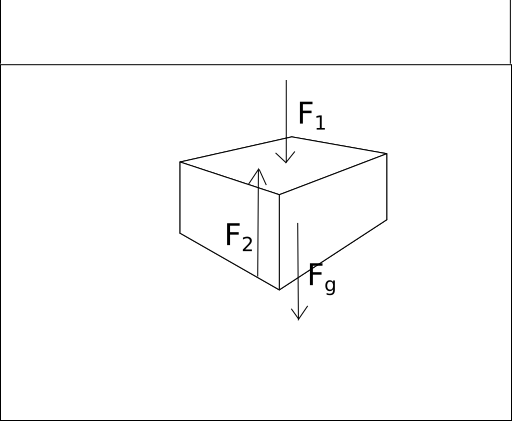
\includegraphics[width=15cm, height=15cm,keepaspectratio=true]{Tekocine.png}
\end{center}
\begin{align*}
	F_1 &\dots \text{sila kapljevina nad kvadromvode}\\
 	F_2 &\dots \text{sila kapljevina pod kvadromvode}\\
 	F_2 &= F_1 + F_g\\
 	p_1 &= \frac{F_1}{S}\\
 	F_1 &= p_1S\\
 	F_2 &= p_2S\\
 	V &= Sh\\
 	F_g = mg &= \rho V g = \rho Shg\\
 	p_2 \cancelto{}{S} &= p_1\cancelto{}{S} + \rho \cancelto{}{S}hg\\
 	p_2 &= p_1 + \rho hg\\
 	p_2-p_1 &= \rho hg\\
 	{\color{bostonuniversityred}\Delta p} &= {\color{bostonuniversityred}\rho hg} \text{hidrostatični tlak}\\
\end{align*}
Če se spustimo za h se tlak poveča za $\Delta p$\\
%\begin{center}
%	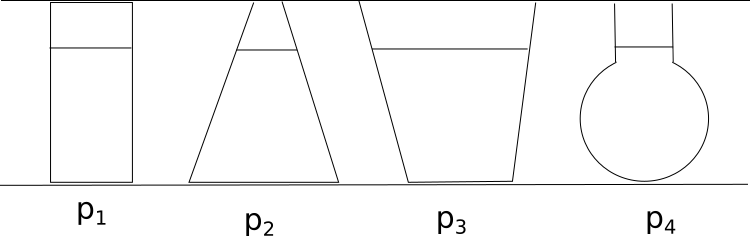
\includegraphics[width=15cm, height=15cm,keepaspectratio=true]{Tekocine2.png}
%\end{center}
\begin{align*}
	p_0 = 1bar &= 10^5 = 10^5 \frac{N}{m^2}\\
	p &= p_0 + \rho gh\\
\end{align*}
\textbf{HIDROSTATIČNI PARADOKS}
\begin{center}
	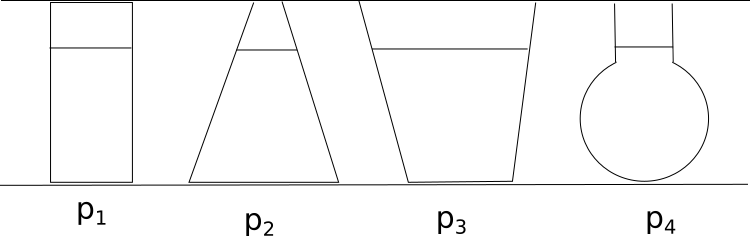
\includegraphics[width=15cm, height=15cm,keepaspectratio=true]{Tekocine2.png}
\end{center}
Tlak na dnu posode je pri vsek enak.\\
\textbf{MERJENJE GOSTOTE KAPLJEVINE Z U CEVKO}
\begin{center}
	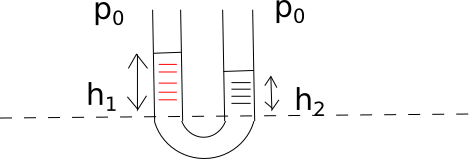
\includegraphics[width=15cm, height=15cm,keepaspectratio=true]{Tekocine3.png}
\end{center}
\begin{align*}
	\Delta p_1 &= \Delta p_2\\
	\rho_1 \cancelto{}{g} h_1 &= \rho_1 \cancelto{}{g} h_1\\
	\rho_1 &= \frac{\rho_2 h_2}{h_1}
\end{align*}
